\documentclass[
	% -- opções da classe memoir --
	12pt,				% tamanho da fonte
	openright,			% capítulos começam em pág ímpar (insere página vazia caso preciso)
	oneside,			% para impressão em verso e anverso. Oposto a oneside
	a4paper,			% tamanho do papel. 
	% -- opções da classe abntex2 --
	%chapter=TITLE,		% títulos de capítulos convertidos em letras maiúsculas
	%section=TITLE,		% títulos de seções convertidos em letras maiúsculas
	%subsection=TITLE,	% títulos de subseções convertidos em letras maiúsculas
	%subsubsection=TITLE,% títulos de subsubseções convertidos em letras maiúsculas
	% -- opções do pacote babel --
	english,			% idioma adicional para hifenização
	french,				% idioma adicional para hifenização
	spanish,			% idioma adicional para hifenização
	brazil				% o último idioma é o principal do documento
	]{abntex2}

% ---
% Pacotes básicos 
% ---
\usepackage{lmodern}			% Usa a fonte Latin Modern			
\usepackage[T1]{fontenc}		    % Selecao de codigos de fonte.
\usepackage[utf8]{inputenc}		% Codificacao do documento (conversão automática dos acentos)
\usepackage{lastpage}			% Usado pela Ficha catalográfica
\usepackage{indentfirst}		    % Indenta o primeiro parágrafo de cada seção.
\usepackage{color}				% Controle das cores
\usepackage{graphicx}			% Inclusão de gráficos
\usepackage{microtype} 			% Para melhorias de justificação
\usepackage{afterpage}
\usepackage{amsmath}            % Pacote para fórmulas matemáticas
\usepackage{amssymb,url}
\usepackage{xcolor,tikz,bm,colortbl}
\usepackage[br]{nicealgo}       % Pacote para criação de algoritmos
\usepackage{customizacoes}
\usepackage{float}
\usepackage{subcaption}
\usepackage{longtable}

% ---
		
% ---
% Pacotes adicionais, usados apenas no âmbito do Modelo Canônico do abnteX2
% ---
\usepackage{lipsum}				% Para geração de dummy text
% ---

% ---
% Pacotes de citações
% ---
\usepackage[brazilian,hyperpageref]{backref}	 % Paginas com as citações na bibl
\usepackage[alf]{abntex2cite}	% Citações padrão ABNT
% --- 
% CONFIGURAÇÕES DE PACOTES
% --- 

% ---
% Configurações do pacote backref
\renewcommand{\familydefault}{\sfdefault}
% Usado sem a opção hyperpageref de backref
\renewcommand{\backrefpagesname}{Citado na(s) página(s):~}
% Texto padrão antes do número das páginas
\renewcommand{\backref}{}
% Define os textos da citação
\renewcommand*{\backrefalt}[4]{
	\ifcase #1 %
		Nenhuma citação no texto.%
	\or
		Citado na página #2.%
	\else
		Citado #1 vezes nas páginas #2.%
	\fi}%
% ---

% ---
% Informações de dados para CAPA e FOLHA DE ROSTO
% ---
\titulo{EXPLORANDO CONTROLE DE INTERAÇÃO EM APLICAÇÃO DE RV PARA DISPOSITIVOS MÓVEIS}
\autor{Amanda Gonçalves Dias}
\local{Bauru}
\data{2016}
\orientador{Prof. Dr. Wilson Yonezawa}
\instituicao{%
  Universidade Estadual Paulista ``Júlio de Mesquita Filho''
  \par
  Faculdade de Ciências
  \par
  Ciência da Computação}
\tipotrabalho{Trabalho de Conclusão de Curso}
% O preambulo deve conter o tipo do trabalho, o objetivo, 
% o nome da instituição e a área de concentração 
\preambulo{Trabalho de Conclusão de Curso do Curso de Ciência da Computação da Universidade Estadual Paulista ``Júlio de Mesquita Filho'', Faculdade de Ciências, Campus Bauru.}
% ---


% ---
% Configurações de aparência do PDF final

% alterando o aspecto da cor azul
\definecolor{blue}{RGB}{41,5,195}

% informações do PDF
\makeatletter
\hypersetup{
     	%pagebackref=true,
		pdftitle={\@title}, 
		pdfauthor={\@author},
    	pdfsubject={\imprimirpreambulo},
	    pdfcreator={LaTeX with abnTeX2},
		pdfkeywords={abnt}{latex}{abntex}{abntex2}{trabalho acadêmico}, 
		colorlinks=true,       		% false: boxed links; true: colored links
    	linkcolor=blue,          	% color of internal links
    	citecolor=blue,        		% color of links to bibliography
    	filecolor=magenta,      		% color of file links
		urlcolor=blue,
		bookmarksdepth=4
}
\makeatother
% --- 

% --- 
% Espaçamentos entre linhas e parágrafos 
% --- 

% O tamanho do parágrafo é dado por:
\setlength{\parindent}{1.3cm}

% Controle do espaçamento entre um parágrafo e outro:
\setlength{\parskip}{0.2cm}  % tente também \onelineskip

% ---
% compila o indice
% ---
\makeindex
% ---

% ----
% Início do documento
% ----
\begin{document}

% Seleciona o idioma do documento (conforme pacotes do babel)
%\selectlanguage{english}
\selectlanguage{brazil}

% Retira espaço extra obsoleto entre as frases.
\frenchspacing 

% ----------------------------------------------------------
% ELEMENTOS PRÉ-TEXTUAIS
% ----------------------------------------------------------
% \pretextual

% ---
% Capa
% ---
\imprimircapa
% ---

% ---
% Folha de rosto
% (o * indica que haverá a ficha bibliográfica)
% ---
\imprimirfolhaderosto
% ---

% ---
% Inserir a ficha bibliografica
% ---

% Isto é um exemplo de Ficha Catalográfica, ou ``Dados internacionais de
% catalogação-na-publicação''. Você pode utilizar este modelo como referência. 
% Porém, provavelmente a biblioteca da sua universidade lhe fornecerá um PDF
% com a ficha catalográfica definitiva após a defesa do trabalho. Quando estiver
% com o documento, salve-o como PDF no diretório do seu projeto e substitua todo
% o conteúdo de implementação deste arquivo pelo comando abaixo:
%
% \begin{fichacatalografica}
%     \includepdf{fig_ficha_catalografica.pdf}
% \end{fichacatalografica}

\begin{fichacatalografica}
	\sffamily
	\vspace*{\fill}					% Posição vertical
	\begin{center}					% Minipage Centralizado
	\fbox{\begin{minipage}[c][8cm]{15.5cm}		% Largura
	\small
	\imprimirautor
	%Sobrenome, Nome do autor
	
	\hspace{0.5cm} \imprimirtitulo  / \imprimirautor. --
	\imprimirlocal, \imprimirdata-
	
	\hspace{0.5cm} \pageref{LastPage} p. : il. (algumas color.) ; 30 cm.\\
	
	\hspace{0.5cm} \imprimirorientadorRotulo~\imprimirorientador\\
	
	\hspace{0.5cm}
	\parbox[t]{\textwidth}{\imprimirtipotrabalho~--~\imprimirinstituicao,
	\imprimirdata.}\\
	
	\hspace{0.5cm}
		1. Tags
		2. Para
		3. A
		4. Ficha
		5. Catalográfica	
	\end{minipage}}
	\end{center}
\end{fichacatalografica}
% ---

% ---
% Inserir folha de aprovação
% ---

% Isto é um exemplo de Folha de aprovação, elemento obrigatório da NBR
% 14724/2011 (seção 4.2.1.3). Você pode utilizar este modelo até a aprovação
% do trabalho. Após isso, substitua todo o conteúdo deste arquivo por uma
% imagem da página assinada pela banca com o comando abaixo:
%
% \includepdf{folhadeaprovacao_final.pdf}
%
\begin{folhadeaprovacao}

  \begin{center}
    {\ABNTEXchapterfont\large\imprimirautor}

    \vspace*{\fill}\vspace*{\fill}
    \begin{center}
      \ABNTEXchapterfont\bfseries\Large\imprimirtitulo
    \end{center}
    \vspace*{\fill}
    
    \hspace{.45\textwidth}
    \begin{minipage}{.5\textwidth}
        \imprimirpreambulo
    \end{minipage}%
    \vspace*{\fill}
   \end{center}
        
   \center Banca Examinadora

   \assinatura{\textbf{\imprimirorientador} \\ Orientador} 
   \assinatura{\textbf{Professor} \\ Convidado 1}
   \assinatura{\textbf{Professor} \\ Convidado 2}
   %\assinatura{\textbf{Professor} \\ Convidado 3}
   %\assinatura{\textbf{Professor} \\ Convidado 4}
      
   \begin{center}
    \vspace*{0.5cm}
    \par
    {Bauru, \_\_\_\_\_ de \_\_\_\_\_\_\_\_\_\_\_ de \_\_\_\_.}
    \vspace*{1cm}
  \end{center}
  
\end{folhadeaprovacao}
% ---

% ---
% Dedicatória
% ---
\begin{dedicatoria}
   \vspace*{\fill}
   \centering
   \noindent
   \textit{Espaço destinado à dedicátoria do texto.} \vspace*{\fill}
\end{dedicatoria}
% ---

% ---
% Agradecimentos
% ---
\begin{agradecimentos}
Espaço destinado aos agradecimentos.
\end{agradecimentos}
% ---

% ---
% Epígrafe
% ---
\begin{epigrafe}
    \vspace*{\fill}
	\begin{flushright}
		\textit{Espaço destinado à epígrafe.}
	\end{flushright}
\end{epigrafe}
% ---

% ---
% RESUMOS
% ---

% resumo em português
\setlength{\absparsep}{18pt} % ajusta o espaçamento dos parágrafos do resumo
\begin{resumo}

Espaço destinado à escrita do resumo.

\textbf{Palavras-chave:} Palavras-chave de seu resumo.
\end{resumo}

% resumo em inglês
\begin{resumo}[Abstract]
 \begin{otherlanguage*}{english}
 
Abstract area.

\textbf{Keywords:} Abstract keywords.
 
 \end{otherlanguage*}
\end{resumo}
% ---

% ---
% inserir lista de ilustrações
% ---
\pdfbookmark[0]{\listfigurename}{lof}
\listoffigures*
\cleardoublepage
% ---

% ---
% inserir lista de tabelas
% ---
\pdfbookmark[0]{\listtablename}{lot}
\listoftables*
\cleardoublepage
% ---

% ---
% inserir lista de abreviaturas e siglas
% ---
% ---

% ---
% inserir o sumario
% ---
\pdfbookmark[0]{\contentsname}{toc}
\tableofcontents*
\cleardoublepage
% ---



% ----------------------------------------------------------
% ELEMENTOS TEXTUAIS
% ----------------------------------------------------------
\pagestyle{simple}

% ----------------------------------------------------------
% Introdução (exemplo de capítulo sem numeração, mas presente no Sumário)
% ----------------------------------------------------------

\chapter{Introdução}
\label{c.introducao}

“Com o advento da realidade virtual e o avanço dos recursos computacionais, as representações interativas e imersivas do imaginário, bem como a reprodução do real, tornaram-se mais fáceis de serem obtidas. ” \cite[p. ~9]{torilivro}

A realidade virtual (RV) vem ganhando espaço em diversos setores como jogos, indústria e educação. Na área de jogos, empresas como Playstation® e Oculus® oferecem um acervo de jogos para as suas respectivas plataformas. Ao procurar por jogos em RV na Google Play, encontram-se algumas opções fornecidas por diversas empresas.

A realidade virtual pode ser utilizada na indústria para avaliar o design de um produto antes do mesmo ser produzido. A The Ford Motor Company é uma das empresas que utilizam a realidade virtual. Com esta tecnologia, é possível visualizar virtualmente tanto o exterior como o interior de um carro a ser produzido e avaliar aspectos de engenharia e design. “A realidade virtual pode ser mais efetiva do que desenvolver o design no mundo real. Só neste ano, designers e engenheiros verificaram mais de 135000 detalhes em 193 protótipos virtuais de veículos” \cite[tradução nossa]{ford}. 

Já na área da educação, a realidade virtual pode ser aplicada através de jogos educativos e aulas imersivas. Imagine uma aula de história passada no local e no tempo de um acontecimento histórico, ou uma aula de astronomia no espaço. Pesquisas como \cite{youngblut} e \cite{carvalho} mostram como a realidade virtual pode ser incorporada na escola.

Para se obter uma experiência em realidade virtual, são necessários capacetes de visualização ou óculos de RV, um display por onde a aplicação irá rodar, um dispositivo de interação e a aplicação em RV. 

Atualmente existem vários modelos de óculos de RV com suporte à realidade virtual, tais como: Oculus Rift da Oculus® com preço estimado de R\$ 4.620,90 e Samsung Gear VR da Samsung® (R\$ 799,00). No entanto, o Google Cardboard da Google® é o que possui preço mais acessível em torno de R\$ 21,97 possuindo atualmente duas versões, cada uma com um meio de interação próprio. Em novembro 2016, a Google lança um novo visualizador denominado Daydream (Figura X). Este visualizador acompanha um controle com comunicação Bluetooth e o capacete de visualização feito com tecido para garantir maior conforto, além de um suporte para fixação do visualizador à cabeça do usuário. Os smartphones compatíveis com o Daydream são os que possuem Android 7.0 ou superior.

\begin{figure}[ht]
	\caption{\small Daydream}
	\centering
	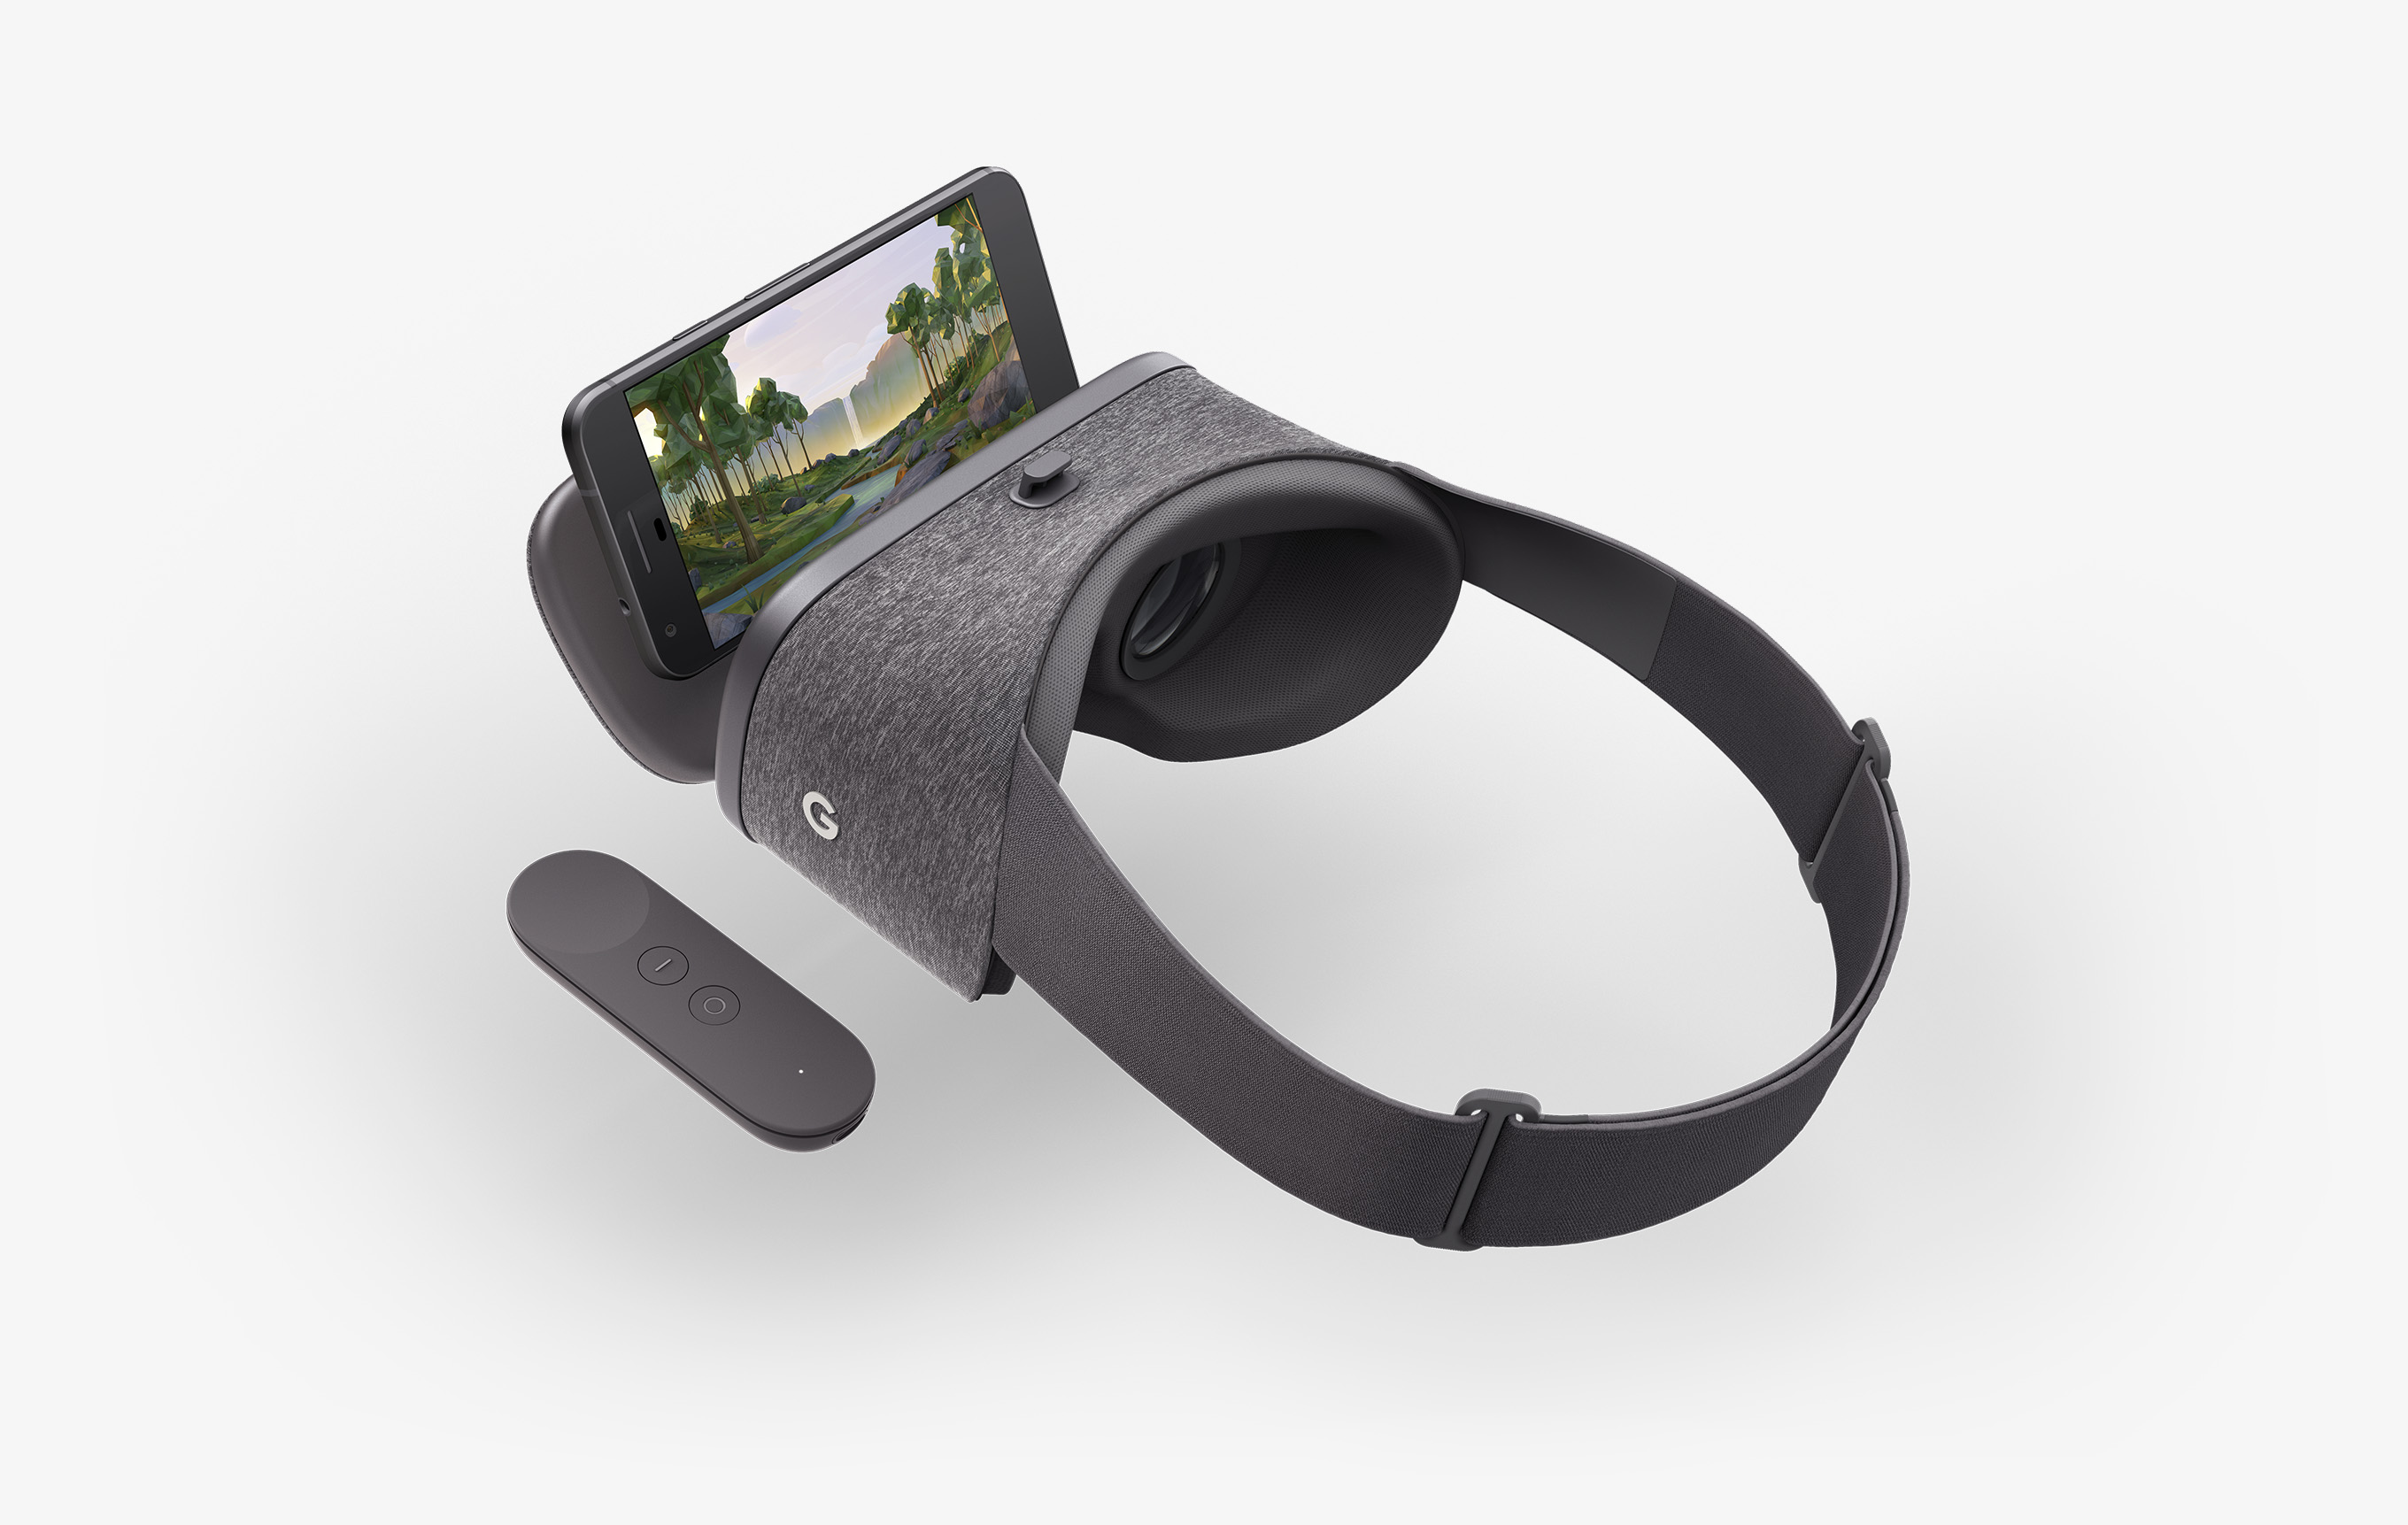
\includegraphics[scale=0.15]{Imagens/daydream.jpg}
	\label{f.daydream}
	\legend{\small Fonte: \cite{daydream}}
\end{figure}

As aplicações em RV podem ser desenvolvidas para plataformas mobile e desktop. A principal diferença entre as duas é a diferença de capacidade de processamento e memória, que são menores nos dispositivos móveis. Para as aplicações desktop utiliza-se óculos de RV como o Oculus Rift para executar a aplicação. Já nas aplicações para dispositivos móveis, é necessário um visualizador como o Google Cardboard por onde o smartphone será encaixado.

A fim de interagir com o ambiente virtual, o usuário pode utilizar a movimentação da cabeça e um controle externo como luvas, mouse 3D, joystick, entre outros. “A necessidade de se fazer uso de aparatos tecnológicos para a interação do usuário com o ambiente virtual provoca restrições, tanto pelo aspecto econômico e tecnológico, quanto pelo desconforto, mas permite ao usuário fazer coisas que antes eram impossíveis ou inviáveis. ” \cite[p. ~3]{torilivro}

Este projeto utiliza óculos de RV e um dispositivo móvel para criar uma aplicação que explora os conceitos da realidade virtual visando explorar diferentes formas de controle de interação.


\section{Problema}
\label{c.problema}

Apesar de o número de aplicações em RV para dispositivos móveis estar em crescimento, este número é pequeno em comparação com aplicações para smartphones sem a tecnologia de RV. Além disso, é atual os estudos de formas de interação com aplicações em RV que possam propiciar conforto, eficácia e conectividade adequada com smartphones. 

O Google Cardboard versão 1 propõe apenas duas formas de interação com o usuário: Movimentação da cabeça e um par de ímãs que quando utilizados representam um toque na tela, seu funcionamento é ilustrado na Figura 2. Já a versão dois não possui ímãs e utiliza o toque na tela como forma de interação como é ilustrado na Figura X. Atualmente, o suporte para a interação via ímã está sendo descontinuado e, por isso, as análises serão feitas utilizando o Google Cardboard versão 2.

\begin{figure}[h]
	\caption{\small Funcionamento do ímã}
	\centering
	\includegraphics[scale=0.7]{Imagens/cardboard.png}
	\label{f.cardboard1}
	\legend{\small Fonte: Elaborada pelo autor.}
\end{figure}

Possuir apenas duas formas de entrada limita as opções de interação do usuário com a aplicação. A empresa Oculus®, vende seus óculos de RV juntamente com um controle de vídeo game, o que garante maior flexibilidade na criação de aplicações em RV. No entanto, a diferença de preço entre o Google Cardboard e o Oculus Rift é alta. 




\section{Justificativa}
\label{c.justificativa}

A realidade virtual é um tema em expansão, objeto de pesquisa de grandes empresas como o Facebook® e a Google®. Logo, investigar formas de utilização desta tecnologia em dispositivos móveis como smartphones é contribuir com conhecimento para a área bem como auxiliar o trabalho de desenvolvedores. 

É interessante apresentar formas diferentes de interação com aplicações em RV e, ao mesmo tempo, obter uma experiência em realidade virtual acessível. O sistema operacional Android oferece bibliotecas que ajudam no tratamento de diversos meios de entradas como Bluetooth e via cabo. Além disso, o celular também possui sensores como acelerômetro e giroscópio que são utilizados para o desenvolvimento de aplicações em RV. Com o auxílio dos recursos mencionados, é possível realizar uma comparação entre diversos tipos de controles físicos, a fim de escolher o mais apropriado para ser utilizado em uma aplicação em RV. 

Por fim, o projeto pode ser realizado com materiais de baixo custo e de fácil acesso, podendo ser encontrados softwares completamente gratuitos.





\chapter{Objetivos}
\label{c.objetivos}

\section{Objetivo Geral}
\label{s.geral}
Explorar formas de interação do usuário em aplicação de RV executada em dispositivos móveis através de um controle externo.

\section{Objetivos Específicos}
\label{s.especifico}
- Identificar os elementos necessários para a criação de uma aplicação em RV.

- Definir as principais restrições na escolha e ferramentas de RV para construção da aplicação.

- Identificar dispositivos físicos como forma de controle na interação entre o usuário e a aplicação RV.

- Realizar a análise dos controles físicos.




\chapter{Método de Pesquisa}
\label{c.metodo}

A Figura 8 apresenta um diagrama com os principais elementos deste projeto de pesquisa. As elipses representam temas ou assuntos. Os retângulos com cantos arredondados, atividades. As setas representam as relações entre diferentes elementos. O cilindro representa uma base de dados de artigos científicos.

\begin{figure}[h]
	\caption{\small Modelo de Pesquisa.}
	\centering
	\includegraphics[scale=0.7]{Imagens/metodologia.png}
	\label{f.metodopesquisa}
	\legend{\small Fonte: Elaborada pelo autor.}
\end{figure}

A pesquisa será dividida em seis etapas. A princípio (fundamentação teórica) será feito um levantamento bibliográfico sobre os tipos de controle físicos que podem ser utilizados no celular, ferramentas para o desenvolvimento de aplicações em realidade virtual e métodos de avaliação para controles físicos.
 
A segunda etapa (preparação do ambiente operacional), envolve a escolha dos software a serem utilizadas com base na exequibilidade do projeto e da acessibilidade das ferramentas, ou seja, devem ser capazes de proporcionar as vias necessárias para o êxito do projeto preferencialmente de forma gratuita e com documentação clara. 

Na terceira fase do projeto (escolha dos controles físicos), será feita a escolha de três tipos de controles que apresentam três diferentes tipos de conexão e iteratividade: via cabo, Bluetooth e toque na tela. 

Na quarta etapa (desenvolvimento da aplicação em RV), será realizado o desenvolvimento da aplicação, se possível com o auxílio de um designer para um visual mais atrativo. Juntamente com o desenvolvimento, serão realizados os testes e correções da aplicação considerando a usabilidade da mesma.
 
A quinta etapa (análise dos controles), verificará se o projeto atingiu os objetivos geral e específicos propostos levando em consideração a análise dos controles em relação as suas características de usabilidade, experiência e funcionalidade. 

Na última (sexta) etapa (relatório de pesquisa), será elaborado o relatório final da pesquisa registrando todos os procedimentos realizados bem como os resultados e conclusões.



\chapter{Fundamentação Teórica}
\label{c.fundamentacao}

\section{Realidade Virtual}
\label{s.rv}
A realidade virtual “é uma interface avançada para aplicações computacionais, que permite ao usuário a movimentação (navegação) e interação em tempo real, em um ambiente tridimensional, podendo fazer uso de dispositivos multissensoriais, para atuação ou \textit{feedback}.” \cite[p. ~7]{torilivro}

A tecnologia de RV permite a imersão do usuário em um ambiente virtual através de um sistema computacional. Com esta tecnologia, é possível enganar os sentidos do usuário para que o mesmo tenha a sensação de que está dentro do ambiente simulado. 

É importante diferenciar os conceitos de RV, realidade aumentada (RA) e virtualidade aumentada (VA). Como explica \citeonline{milgram}, o ambiente propiciado pela RV é totalmente sintético, ou virtual, e pode ou não imitar o mundo real. Já ambientes em RA intercalam o real e o virtual tornando o capacete de visualização “transparente”, acrescentando elementos virtuais no ambiente real. Por fim, a VA traz ambientes virtuais com alguns elementos reais como a representação das mãos do usuário, por exemplo. A Figura ~\ref{f.milgram} mostra uma relação entre as tecnologias descritas acima.

\begin{figure}[ht]
	\caption{\small \textit{Virtual Reality Continuum}}
	\centering
	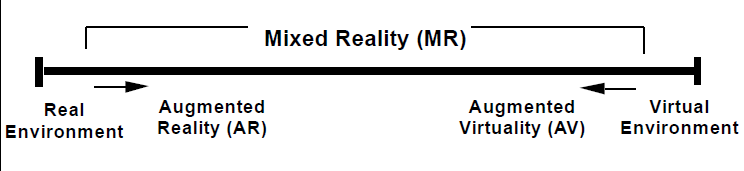
\includegraphics[scale=0.7]{Imagens/milgram.png}
	\label{f.milgram}
	\legend{\small Fonte: \citeonline{milgram}}
\end{figure}

Para se criar a sensação de imersão propiciada pela RV, é utilizada a estereoscopia (Figura ~\ref{f.estereoscopia}), ou seja, é gerada uma imagem para cada olho. Esta técnica faz com que o cérebro interprete as imagens como uma. \citeonline[p. ~221]{siscoutto} explicam que a importância da estereoscopia ou visão binocular pode ser averiguada na prática ao fechar um olho e tentar exercer atividades cotidianas desta forma. O que será observado é que a visão monocular, torna o simples ato de pegar um objeto sobre a mesa uma tarefa difícil pois esta visão conta com uma percepção rudimentar de profundidade.

\begin{figure}[H]
	\caption{\small Estereoscopia}
	\centering
	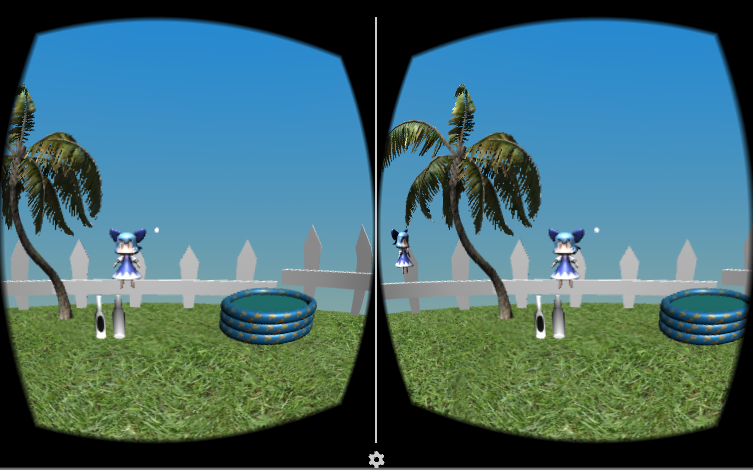
\includegraphics[scale=0.7]{Imagens/estereoscopia.png}
	\label{f.estereoscopia}
	\legend{\small Fonte: Elaborada pelo autor.}
\end{figure}

Além da estereoscopia, a navegação e a interação com o ambiente virtual também são características da RV. De acordo com \citeonline[p. ~9]{torilivro}, a navegação em espaços tridimensionais dá-se por movimentos de translação e de rotação ao longo dos três eixos (X, Y, Z) resultando em 6 graus de liberdade (3 de rotação e 3 de translação) como mostra a Figura ~\ref{f.grausliberdade}. 

\begin{figure}[ht]
	\caption{\small Graus de Liberdade}
	\centering
	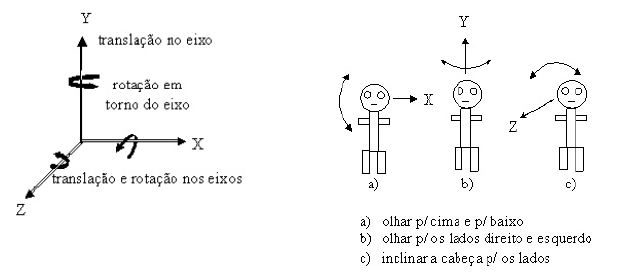
\includegraphics[scale=1.0]{Imagens/grausliberdade.png}
	\label{f.grausliberdade}
	\legend{\small Fonte: \citeonline{torilivro}.}
\end{figure}

O conceito de realidade virtual, segundo \citeonline[p. ~98]{rodrigues}, apesar de existir a mais de vinte anos, alcançou popularidade apenas recentemente. Este fato se deu devido a diminuição do custo para a sua implementação.

\subsection{Fatores Fisiológicos}
\label{ss.fatoresfisiologicos}
Quando tenta-se criar uma simulação imersiva, é importante ter em mente alguns fatores fisiológicos que não são levados em consideração em aplicações não imersivas. Estes fatores, quando não implementados corretamente, podem levar ao chamado \textit{motion sickness} ou VR \textit{sickness} que, segundo a \citeonline{vrsickness}, é a sensação de náusea devido à disparidade entre o que é sentido e o que é esperado sentir. Esta disparidade faz com que nosso corpo se sinta “envenenado” causando desconforto ao usuário. 

De acordo com a \citeonline{oculus}, encontrar fatores que contribuem para o \textit{motion sickness} pode ser complicado pois as pessoas sentem este desconforto de forma desigual. Enquanto um pode sentir náusea em um curto período de exposição à uma aplicação em RV, outro pode não sentir nada após um longo período. Outro empecilho é a possibilidade de se acostumar ao ambiente imersivo e não sentir mais o desconforto. Por isso, não é recomendado que os desenvolvedores da aplicação determinem quais são ou não fatores causadores do VR \textit{sickness}. 

Como alternativa, é recomendado evitar algumas características que, segundo a \citeonline{oculus} demonstraram serem fatores contribuintes para o desconforto do usuário. Um destes fatores é a aceleração da câmera. Diferente de aplicações não imersivas, a movimentação do usuário pela aplicação deve ser analisada com cuidado pois, como o usuário está parado enquanto o personagem está se movimentando, ocorre a discrepância de sensações resultando no desconforto.

Outro fator é o grau de controle do usuário sobre o ambiente. Ao travar a tela para que alguma mensagem seja visualizada ou realizar a rotação da câmera para algum ponto, é retirado o poder de controle do usuário, o que também é considerado um fator facilitador do VR \textit{sickness}.

A distância dos objetos à câmera também deve ser analisada. O usuário deve ser capaz de ler uma mensagem em frente à câmera com facilidade, o posicionamento incorreto da mensagem pode causar incômodo ao usuário dificultando a leitura.

Tendo em vista a redução do VR \textit{sickness} foram criados guias de boas práticas para serem levados em consideração ao desenvolver aplicações em RV.

\subsection{Boas Práticas}
\label{ss.boaspraticas}

Para auxiliar desenvolvedores, a Google® lançou um aplicativo para dispositivos Android denominado \textit{Cardboard Design Lab} (Figura ~\ref{f.designlab}). Neste aplicativo, o usuário pode aprender técnicas que são classificadas em duas categorias: criação e imersão. A primeira categoria, segundo \citeonline{hopkins}, foca nos princípios básicos da criação de aplicações em RV. Já a segunda categoria é mais exploratória, levando em consideração teoria e experiências através do aplicativo. Em cada categoria são fornecidas lições onde o usuário verá cenários onde as técnicas são aplicadas e, em alguns casos, sentirá o \textit{motion sickness} quando determinado cuidado não for tomado. 

\begin{figure}[H]
	\caption{\small Cardboard Design Lab}
	\centering
	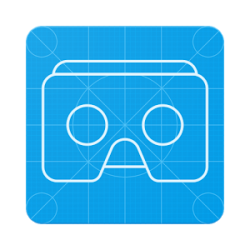
\includegraphics[scale=0.5]{Imagens/designlab.png}
	\label{f.designlab}
	\legend{\small Fonte: \citeonline{designlab}}
\end{figure}

Primeiramente, o aplicativo mostra a necessidade de se utilizar o retículo - círculo no centro da tela que aumenta o seu raio ao passar por algum objeto, variando o seu posicionamento com base na movimentação de cabeça do usuário. Como ainda não existe o rastreamento do olho do usuário em aplicações de RV para dispositivos móveis, é muito difícil saber para onde a cabeça está apontando quando o retículo é inexistente, tornando a seleção de objetos em um cenário muito mais complicada. 

A distância entre o usuário e caixas de textos que eventualmente aparecem na tela é outro fator a ser levado em consideração. Segundo ainda o guia, uma distância confortável para a leitura é de três metros à frente da câmera. 

A movimentação do usuário no cenário pode ser feita de algumas maneiras para que não se cause o desconforto. Um modo é mover a câmera de forma constante, sem variações de aceleração. Também é possível realizar o desvanecer ou \textit{fade} da tela, que é quando a imagem do cenário desaparece e outro cenário reaparece. Segundo \citeonline{tom}, se este clique da tela estiver na frequência correta, o nosso cérebro interpreta esta mudança como um piscar dos olhos, tornando a transição imperceptível. 

Como um dos principais conceitos da realidade virtual é a imersão do usuário, o mesmo deve se sentir confortável no ambiente e, para que isso ocorra, a escala dos objetos no ambiente imersivo deve corresponder ao máximo a realidade, para que o usuário se sinta no mesmo “mundo” do espaço virtual. O mesmo vale para os sons presentes na aplicação, que devem considerar o posicionamento do usuário. Além disso, utilizar pontos de referência no ambiente evitam que o usuário se sinta desorientado. Quanto ao controle do usuário, uma recomendação geral é nunca travar a cena. Ou seja, é importante que a movimentação da cabeça esteja sempre habilitada.

Para auxiliar o usuário a navegar através da aplicação, pode-se utilizar recursos como pontos de luz para indicar o caminho a ser seguido, além de sinalizações para indicar onde o usuário deveria olhar. A última recomendação do aplicativo apresentado pela Google® é criar aplicações visualmente agradáveis como na Figura ~\ref{f.makeitbeatiful} a fim de maximizar a ilusão de imersão do usuário. 

\begin{figure}[h]
	\caption{\small Visual Agradável}
	\centering
	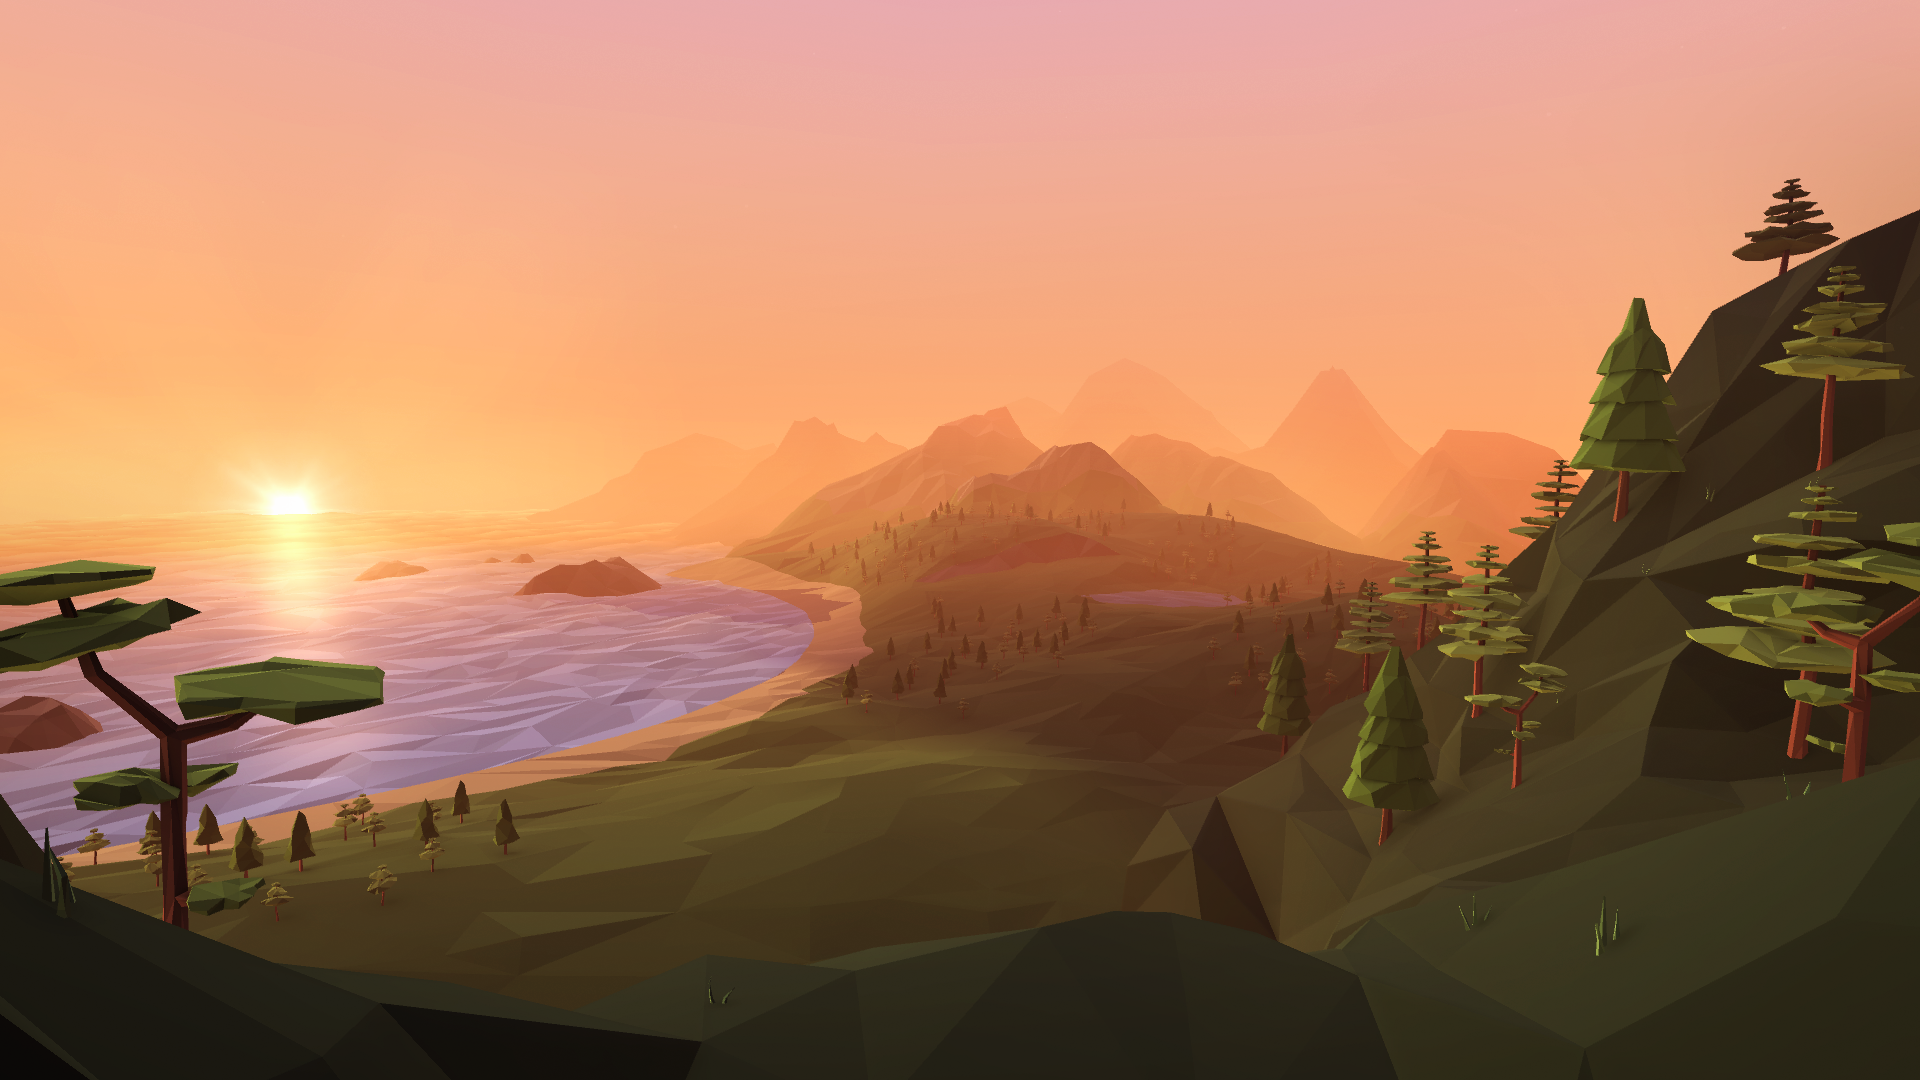
\includegraphics[scale=0.2]{Imagens/makeitbeautiful.png}
	\label{f.makeitbeatiful}
	\legend{\small Fonte: \citeonline{hopkins}.}
\end{figure}


\section{Dispositivos de Controle de Interação Homem/Máquina}
\label{s.dispositivos}

Com a inserção das máquinas no cotidiano das pessoas, surgiu uma área de estudos multidisciplinar que visa compreender as interações entre o usuário e o computador denominada \textit{Human Computer Interaction} (Interação Humano-Computador). Segundo \citeonline[p. ~3]{dix}, entende-se por usuário um indivíduo ou grupo de pessoas trabalhando juntas ou uma sequência de usuários em uma organização. O usuário é qualquer um que está tentando cumprir um objetivo utilizando a tecnologia. O computador representa qualquer tecnologia inclusive partes não computadorizadas como outras pessoas. Por interação entende-se qualquer meio de comunicação entre o usuário e a máquina.  

Em relação a área de estudo Interação Humano-Computador, é possível citar um grande número de dispositivos que podem ser considerados computador pelos quais o usuário irá interagir a fim de realizar algum objetivo. Como exemplos, existem os dispositivos de entrada como dispositivos de texto, de posicionamento e indicação e os dispositivos de saída como a tela do computador ou celular. 

O teclado é um dos dispositivos de entrada de texto mais comuns. Os teclados funcionam com o pressionar das teclas, fechando a conexão e fazendo com que um código de caractere seja enviado ao computador. Atualmente, a maioria dos teclados seguem o layout de teclas QWERT (Figura ~\ref{f.qwert}) que, apesar de não ser considerada a distribuição ótima, foi implementado pois o teclado baseou-se nas máquinas de escrever onde o posicionamento das teclas levava em consideração letras que possivelmente seriam combinadas. Estas eram colocadas distantes no teclado para se evitar que os braços se aglomerassem de um lado da máquina. Reconhecedor de voz e de escrita também podem ser considerados dispositivos de entrada de texto.

\begin{figure}[H]
	\caption{\small Teclado padrão QWERT}
	\centering
	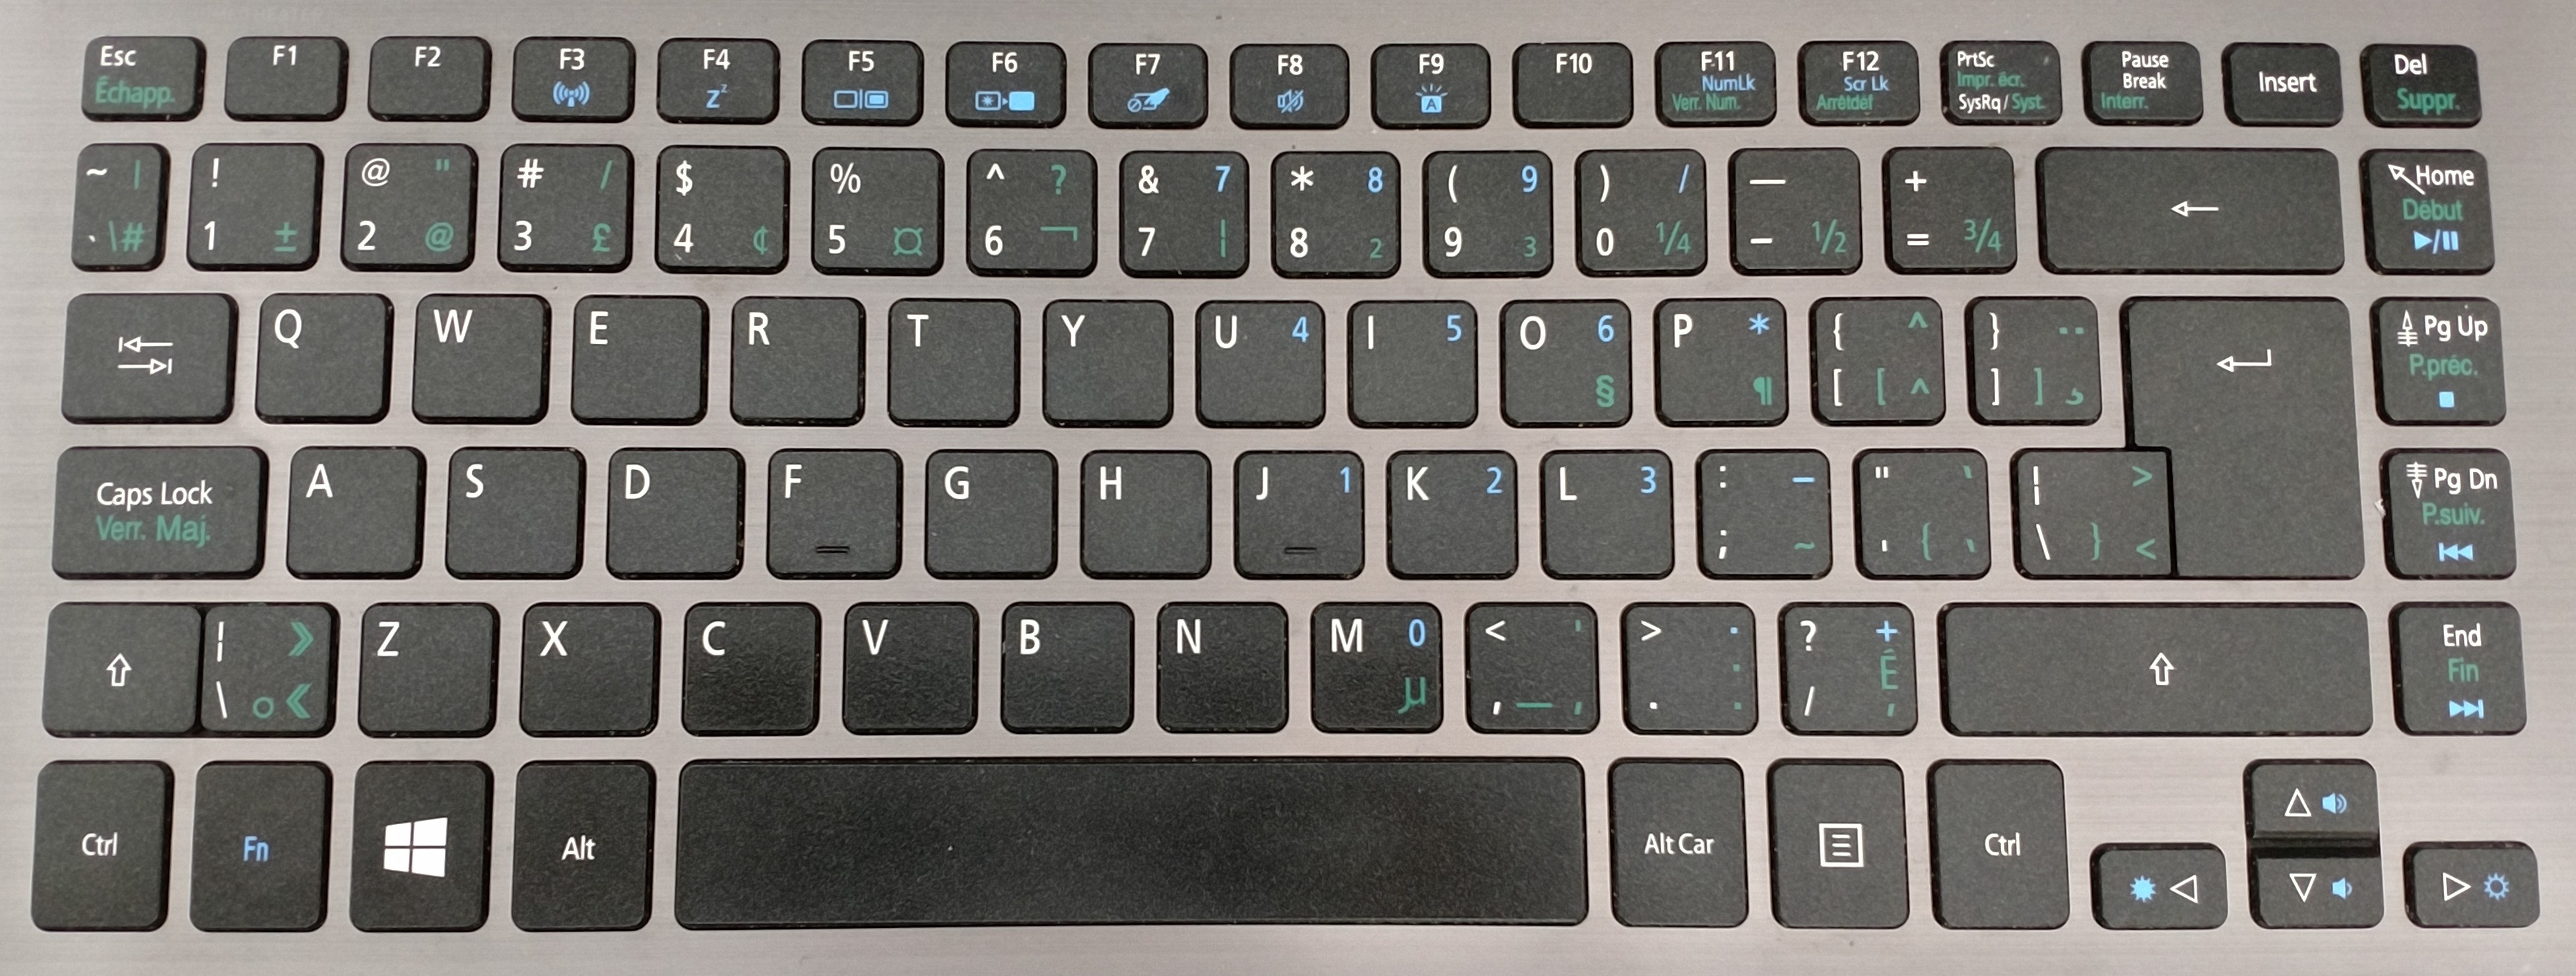
\includegraphics[height= 5cm]{Imagens/qwert.jpg}
	\label{f.qwert}
	\legend{\small Fonte: Elaborada pelo autor.}
\end{figure}

\citeonline{dix} descrevem os dispositivos de posicionamento e indicação dando o exemplo do mouse como um destes dispositivos. Outros dispositivos como os \textit{joysticks}, telas \textit{touchscreens}, \textit{touchpads} e as setas do teclado também estão nesta categoria.  Quando o contexto é um ambiente 3D, o mouse 3D, as luvas de dados (luvas com fibras ópticas ao longo dos dedos que detectam o ângulo das articulações) e capacetes de realidade virtual são alguns dos dispositivos desta categoria. 

Assim como os computadores \textit{desktops}, outros dispositivos de interação homem-máquina também tiveram a sua evolução ao longo do tempo. As telas \textit{touchscreens} sendo utilizadas como mouse em celulares e \textit{desktops}, o desenvolvimento de telas 3D e capacetes em realidade virtual capazes de criar ambientes imersivos são exemplos desta evolução. O crescimento dos dispositivos móveis acarretou no aumento do número de dispositivos de interação com estes minicomputadores como telas de alta densidade, capacidade gráfica 3D e sensores. Com a anexação de sensores como o acelerômetro e giroscópio foi possível a incorporação de aplicações em realidade virtual em dispositivos móveis.

\subsection{Acelerômetro e Giroscópio}
\label{ss.acelerometrogiroscopio}

Segundo \citeonline{bergstrom}, os sensores de inércia como os acelerômetros e os giroscópios possuem a função de converter um fenômeno físico em um sinal mensurável. O acelerômetro é normalmente definido num plano cartesiano e mede a força cinética causada por uma aceleração linear. Já os giroscópios medem a velocidade angular de uma rotação sob seu eixo primário.

De acordo com a empresa \citeonline{dimension}, a aceleração medida pelo acelerômetro pode ser estática ou dinâmica. A gravidade é um exemplo de força estática e uma das vantagens de medir esta aceleração é a possibilidade de descobrir o ângulo do dispositivo em relação à Terra. Já a medição da aceleração dinâmica revela em qual direção o dispositivo está se movendo. 

Quando inseridos em \textit{smartphones}, os acelerômetros podem ser utilizados para funções diversas que vão desde realizar a rotação da tela de acordo com a orientação em que o dispositivo se encontra até reconhecer movimentos do usuário como o caminhar e a movimentação da cabeça. 

Já os giroscópios funcionam como uma bússola indicando a posição do dispositivo no espaço. Estes medem a taxa de rotação ao longo dos três eixos do sensor, onde a rotação é positiva no sentido anti-horário. Aplicações em RV utilizam as informações do giroscópio para saber para onde o usuário está olhando através da rotação da cabeça. \cite{android}

\subsection{Computação Móvel}
\label{ss.computacaomovel}

Tendo em vista a popularidade e o avanço dos dispositivos móveis, é importante entender o significado de computação móvel a fim de se criar aplicações que podem ser executadas neste contexto. Para compreender o conceito de computação móvel, é preciso definir o que é mobilidade.

\begin{citacao}
	"No contexto da computação móvel, mobilidade se refere ao uso pelas pessoas de dispositivos móveis portáveis funcionalmente poderosos que ofereçam a capacidade de realizar facilmente um conjunto de funções de aplicação, sendo também capazes de conectar-se, obter dados e fornecê-los a outros usuários, aplicações e sistemas." \cite[p. ~1]{lee}
\end{citacao}

Com os avanços do hardware dos computadores, foi possível criar aparelhos cada vez menores e, apesar dos dispositivos móveis serem portáteis, diferentes aparelhos possuem diferentes níveis de portabilidade. De acordo com \citeonline{lee}, a portabilidade é afetada pelos fatores tamanho e peso do dispositivo (considerando seus acessórios). Logo, um \textit{smartphone} que cabe em uma mão é mais portátil do que um laptop que necessita de uma bolsa ou maleta, por exemplo. 

Contudo, além da portabilidade também é necessário levar em consideração a usabilidade, a funcionalidade e a conectividade dos dispositivos. \citeonline{lee} definem a usabilidade como algo que depende do usuário, ambiente e as características do dispositivo enquanto que a funcionalidade é dividida nas categorias aplicações independentes, ou seja, o usuário não tem contato com outro usuário ou sistema, e dependentes, quando é necessário conectar-se a outro usuário ou sistema. Em relação à conectividade é importante apontar que um dispositivo móvel não possui necessariamente uma conexão sem fio.

Quanto à usabilidade é natural que um dispositivo móvel como um laptop seja mais facilmente transportado por um adulto do que por uma criança. Assim como certos usuários não possuem facilidade para interagir com certos dispositivos. Outros fatores como a característica do ambiente e as características do dispositivo afetam na escolha do dispositivo com melhor usabilidade. 

Em resumo, a computação móvel é definida a partir de diversos fatores. Diferentes tipos de dispositivos móveis possuem características distintas que, apesar de serem consideradas móveis, apresentam certas diferenças que devem ser levadas em consideração para se escolher o dispositivo mais adequado para determinada aplicação.

\textit{Smartphones} são dispositivos móveis que estão se tornando cada vez mais potentes. A evolução dos \textit{smartphones} permitiu a conexão de diversos dispositivos que aumentam ainda mais as possibilidades de interação homem-máquina. 

 	
\chapter{Ferramentas}
\label{c.ferramentas}

\section{Unity}
\label{s.unity}
Tendo em vista que a aplicação será feita em um dispositivo com sistema operacional Android, a ferramenta de desenvolvimento escolhida deverá oferecer suporte para este tipo de dispositivo. A Google® oferece recursos para desenvolvimento em RV para Android e possui duas opções de ferramentas: SDK do Android, SDK do Unity, SDK do iOS e SDK do Unreal Engine 4. \cite{googledocumentacao} 

As opções contam com um projeto exemplo e materiais explicativos sobre o desenvolvimento de aplicações em realidade virtual. Além disso, a Google® oferece guias de boas práticas para a criação de aplicações em RV. 

Após análise, foi escolhido o SDK do Unity para o desenvolvimento da aplicação pois o mesmo oferece um ambiente gráfico intuitivo que não depende somente do código puro. Além disso, o Unity possibilita a exportação da aplicação para múltiplas plataformas de forma simples e rápida.

Segundo a empresa \citeonline{unitynumbers}, esta feramenta é o principal software de desenvolvimento de jogos em escala global com 5 bilhões de jogos feitos em Unity baixados no 3º semestre de 2016 e 770 milhões de pessoas que jogam jogos feitos com a ferramenta. Na área da RV, é estimado que 90\% dos jogos desenvolvidos para o Samsung Gear VR e 53\% dos jogos desenvolvidos para o Oculus Rift foram feitos através do Unity.

O ambiente de desenvolvimento do Unity pode ser visualizado na Figura X, onde o menu do lado esquerdo contém os objetos presentes na cena, o centro contém a cena em si e o lado direito as propriedades dos objetos selecionados. Esta disposição dos elementos pode ser personalizada pelo usuário. Em cada elemento da cena, é possível adicionar scripts que definirão as ações sobre os objetos, podendo ser decorrentes do input do usuário e do estado da aplicação em geral. O Unity utiliza duas linguagens de programação para a criação de scripts: C\# e UnityScript.  

\begin{figure}[h]
	\caption{\small Unity}
	\centering
	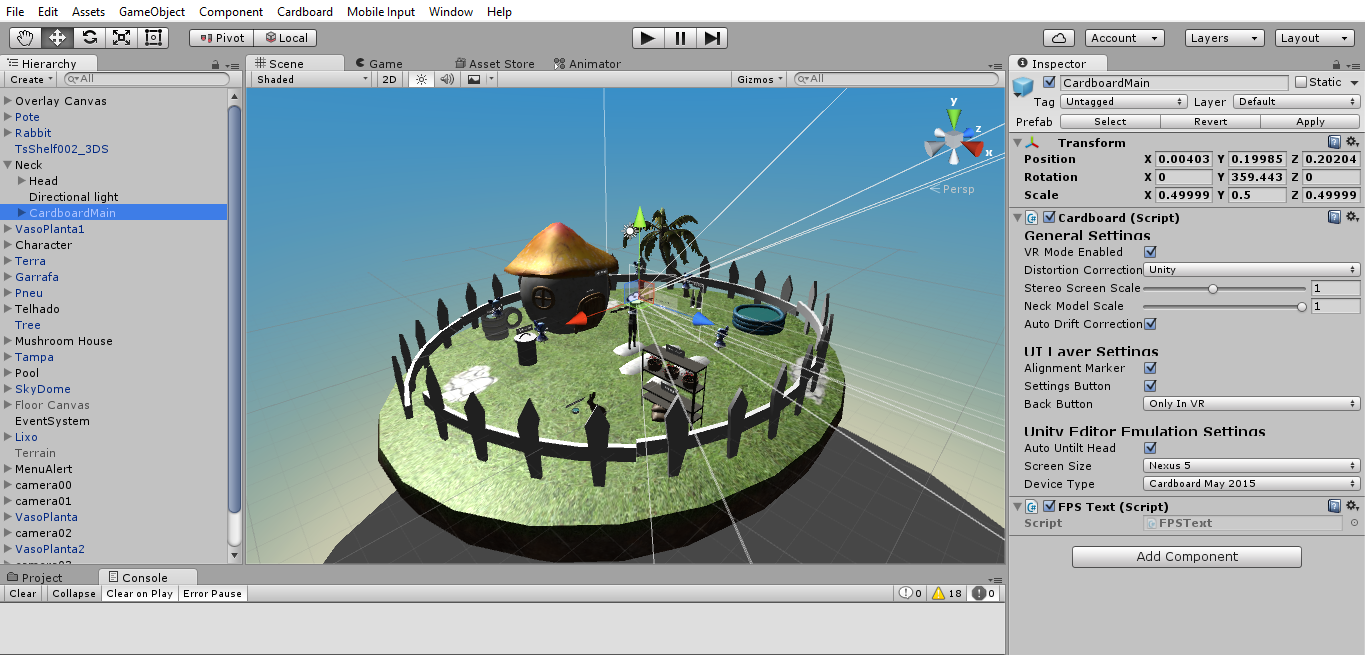
\includegraphics[height= 8cm]{Imagens/unity.png}
	\label{f.unity}
	\legend{\small Fonte: Elaborada pelo autor.}
\end{figure}

A fim de criar uma imagem para cada olho e proporcionar a sensação de imersão, são utilizadas duas câmeras (uma para cada olho). De acordo com a documentação oficial do Unity, para mover ou girar a câmera, é preciso anexar as mesmas à um objeto. Desta forma, ao movimentar o objeto, as câmeras refletirão o movimento. 

\subsection{Integração Unity e Google VR}
\label{ss.unitygoogle}

Para facilitar o desenvolvimento de aplicações para o Google Cardboard e o Daydream, o Unity possui integração nativa com o Google VR. Para recursos adicionais, a Google disponibiliza a Google VR SDK (Coleção de desenvolvimento de software) que requere a versão 5.2.1 ou superior do Unity e traz recursos como áudio espacial, suporte para o controle Daydream, ferramentas utilitárias e exemplos.  Segundo a \citeonline{googleunity}, a integração do Unity com o Google VR possibilita a localização da cabeça do usuário, renderização stereo, entre outros. 

\section{Capacetes de Visualização}
\label{s.capacetes}

Para este projeto, serão utilizados dois capacetes de visualização: o Google Cardboard (Figura X) e o VR Box (Figura X). Ambos foram escolhidos devido ao baixo custo e por utilizarem um smartphone como display. 

\begin{figure}[H]
	
	\begin{minipage}{.5\textwidth}{
			\centering
			\captionof{figure}{\small Google Cardboard}
			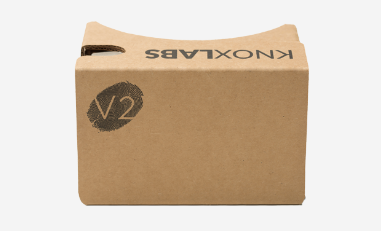
\includegraphics[height=4cm]{Imagens/googlecardboard.png}		
			\label{f.googlecardboard}	
			\legend{\small Fonte: \cite{googlecardboard}.}
		}
	\end{minipage}
	\begin{minipage}{.5\textwidth}{
			\centering
			\captionof{figure}{\small VR Box}
			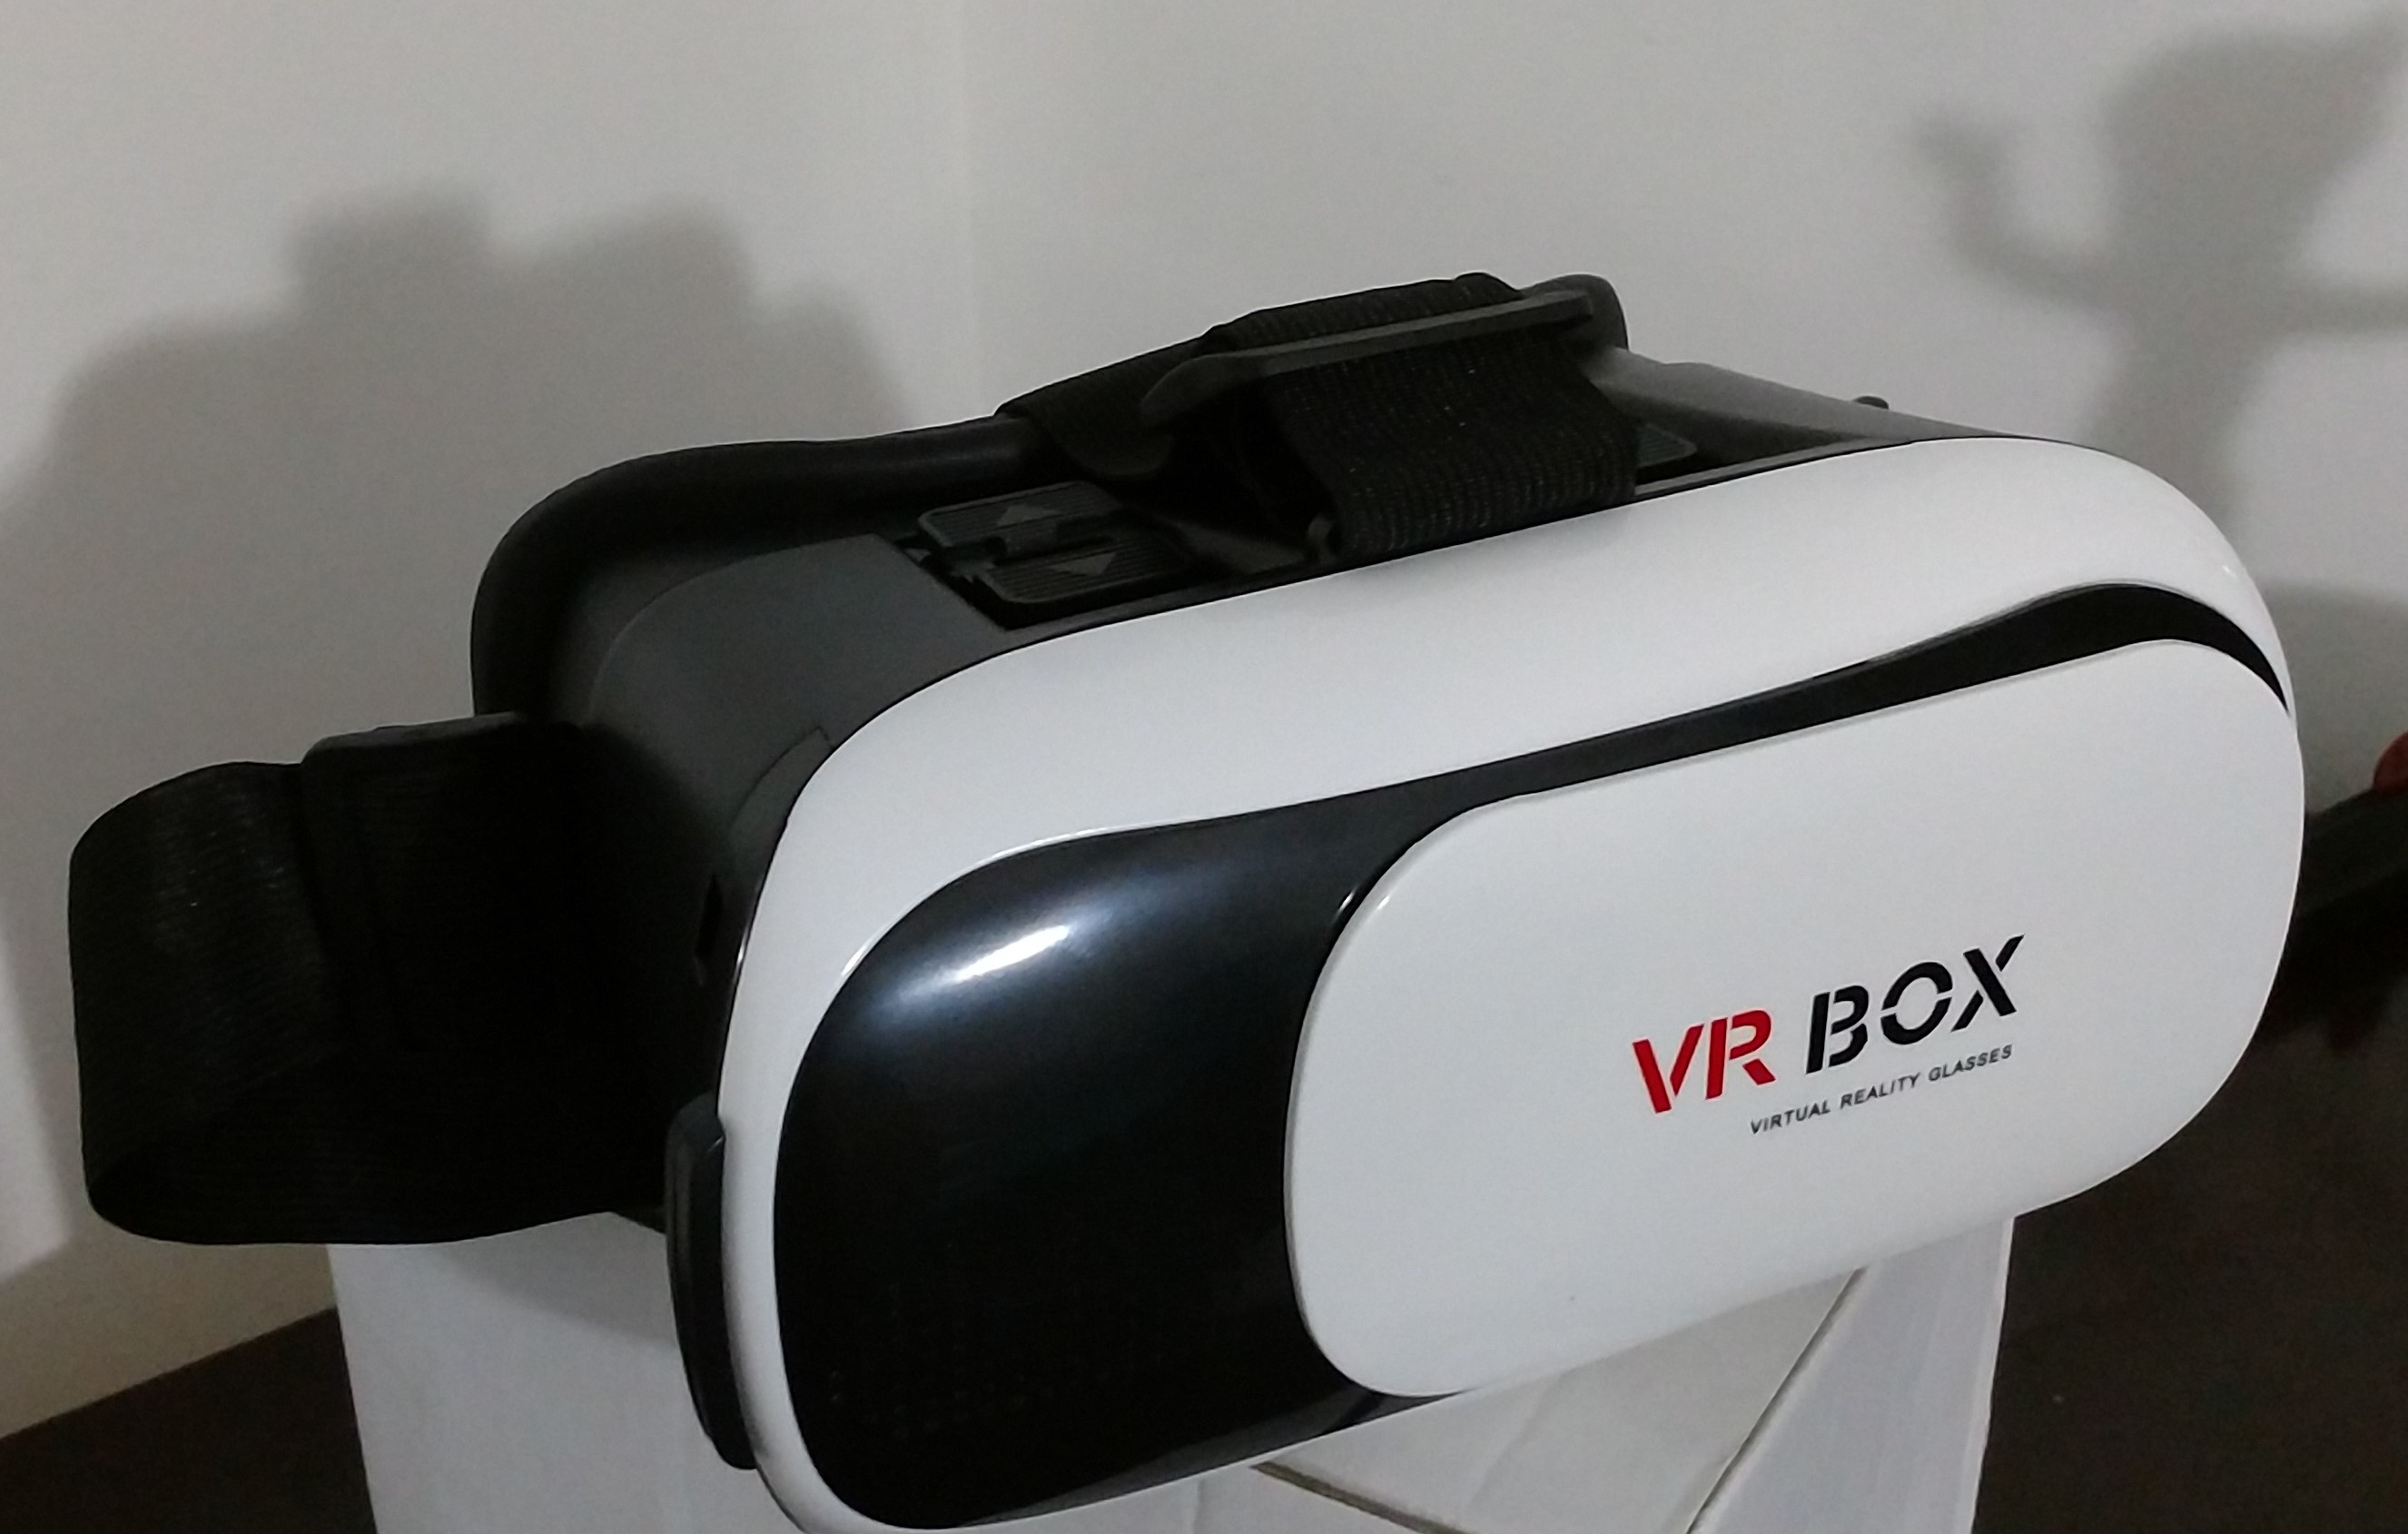
\includegraphics[height=4cm]{Imagens/vrbox.jpg}		
			\label{f.vrbox}
			\legend{\small Fonte: Elaborada pelo autor.}	
		}
	\end{minipage}
	
\end{figure}


O Google Cardboard proporciona experiências de imersão para todas as pessoas de uma forma simples e barata. Você pode montar seu próprio visualizador ou comprar um visualizador certificado com o selo “Funciona com o Google Cardboard” para ficar a apenas um passo de ter a realidade virtual no seu smartphone. \cite{googlecardboard}

O Google Cardboard 2.0 pode ser adquirido em diversos modelos como mostra a Figura X. Apesar da primeira versão do Cardboard possuir um modelo pra a montagem do visualizador, o modelo da segunda versão ainda não foi disponibilizado pela empresa, apesar de existir modelos de outras fontes.

\begin{figure}[h]
	\caption{\small Google Cardboard V2 Modelos}
	\centering
	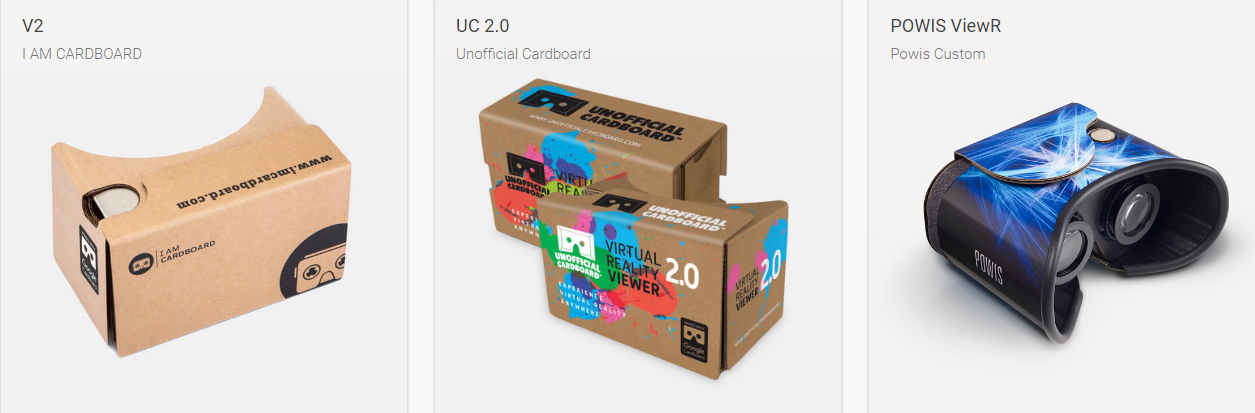
\includegraphics[scale=0.5]{Imagens/modelos.png}
	\label{f.modelos}
	\legend{\small Fonte: \cite{googlecardboard}.}
\end{figure}

Originalmente, o Google Cardboard não possui suporte para a fixação na cabeça do usuário, ou seja, o usuário terá que segurar o visualizador durante toda a experiência em RV, o que dificulta o uso de controle externos já que os mesmos deverão ser utilizados com somente uma das mãos do usuário. O visualizador comporta smartphones de 4.7 até 5.5 polegadas.

O visualizador VR Box vem acompanhado de um controle com comunicação Bluetooth além de já possuir o suporte para cabeça. Diferentemente do Google Cardboard, o VR Box possui um compartimento ajustável para a inserção do smartphone (Figura X), possibilitando uma melhor fixação de smartphones de diversos tamanhos (4,7 até 6 polegadas) ao visualizador.

\begin{figure}[H]
	\caption{\small Compartimento para smartphone}
	\centering
	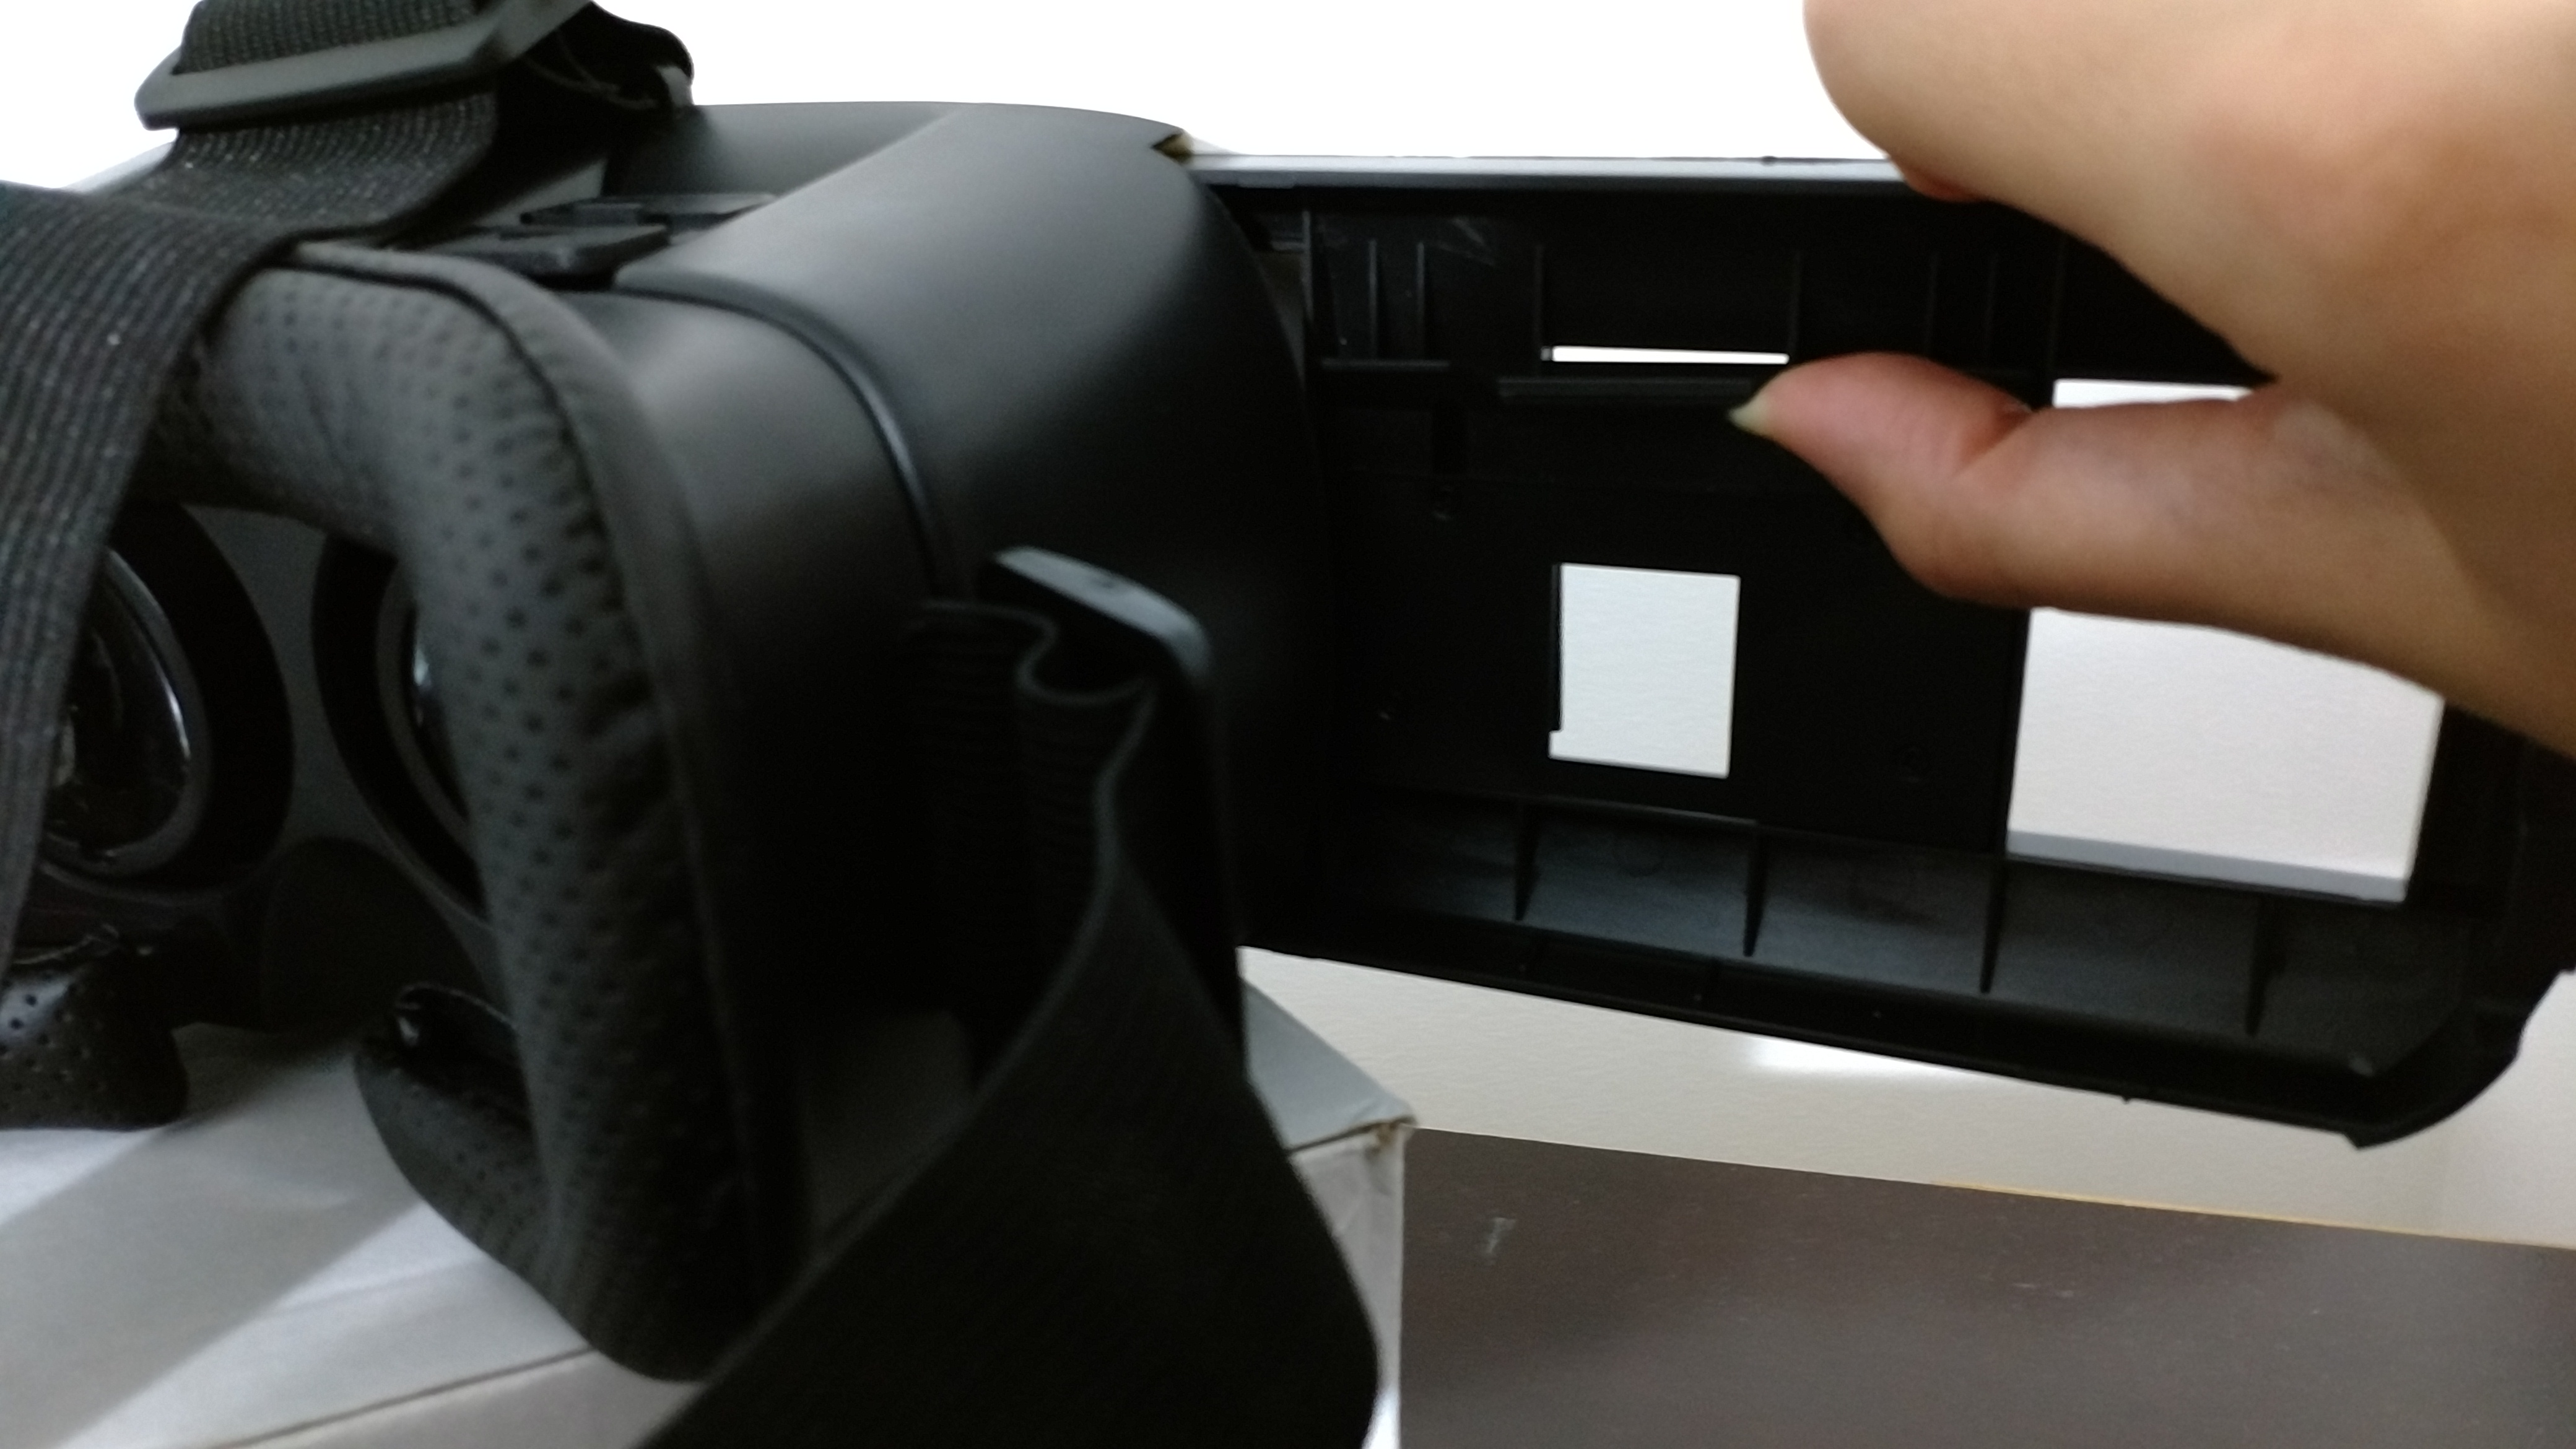
\includegraphics[height=5cm]{Imagens/extensor.jpg}
	\label{f.extensor}
	\legend{\small Fonte: Elaborada pelo autor.}
\end{figure}



\section{Dispositivo Móvel}
\label{s.dispositivomovel}

Para se obter uma experiência completa em RV, é necessário que o dispositivo móvel possua giroscópio e acelerômetro. Ao adquirir o Google Cardboard é necessário observar as especificações do visualizador para saber quais tamanhos de telas são suportadas. 

Os testes previstos neste projeto serão realizados em um smartphone da Motorola, modelo Moto Z. As especificações principais deste dispositivo podem ser visualizadas na Tabela X




\chapter{Aplicação}
\label{c.aplicacao}

\section{Descrição da Aplicação}
\label{s.descricao}

Na aplicação a ser desenvolvida, o usuário irá explorar uma área que conterá vários objetos. O objetivo do usuário será de se movimentar no espaço através de um controle físico, procurar objetos específicos ao redor movimentando a cabeça e executar ações sobre os mesmos.

A fim de contextualizar o usuário no ambiente e definir os objetos que receberão ações, a aplicação terá como tema o mosquito Aedes aegypti, onde o usuário terá que eliminar os focos do mosquito no quintal de uma casa. 

O \citeonline{riodejaneiro} publicou em seu website os lugares propícios para a reprodução do mosquito juntamente com as precauções que as pessoas devem tomar para a eliminação do Aedes aegypti. Os usuários da aplicação deverão realizar seis das quinze providências fornecidas pelo website que são:

•	Coloque areia no prato dos vasos de plantas.

•	Mantenha o saco de lixo bem fechado e fora do alcance de animais até o recolhimento pelo serviço de limpeza urbana. Não jogue lixo em terrenos baldios.

•	Troque diariamente a água dos bebedouros de animais e aves e limpe-os com escova ou bucha.

•	Entregue seus pneus velhos ao serviço de limpeza urbana ou guarde-os sem água em local coberto e abrigados da chuva.

•	Guarde as garrafas vazias sempre de cabeça para baixo e de preferência em local coberto.

•	Limpe constantemente as calhas, remova tudo que possa impedir a passagem da água, a laje e a piscina de sua casa

\section{Ações}
\label{s.acoes}

O usuário contará com cinco ações dentro da aplicação: andar, agachar, focar, selecionar e abrir o menu. Os caminhos possíveis que o usuário poderá percorrer serão determinados por objetos que servirão como guias dentro da aplicação. Ao selecionar os guias, o usuário irá caminhar até os mesmos, podendo atingir seis posições no cenário como mostra a Figura X.

\begin{figure}[h]
	\caption{\small Posições possíveis na aplicação}
	\centering
	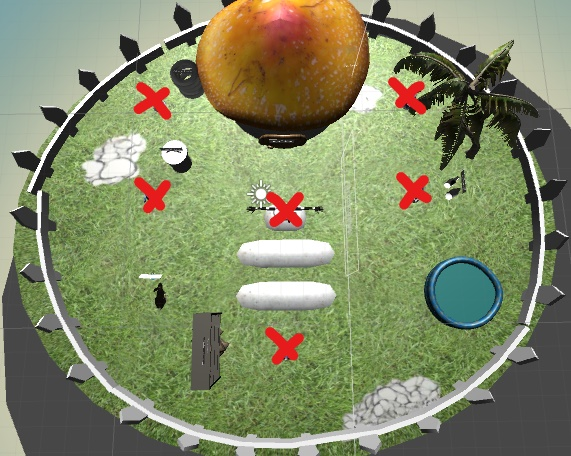
\includegraphics[scale=0.50]{Imagens/posicoes.jpg}
	\label{f.posicoes}
	\legend{\small Fonte: Elaborada pelo autor.}
\end{figure}

Os objetos que poderão sofrer ações possuem um menu que é acionado enquanto o usuário foca o objeto. Este menu mostrará qual ação é permitida para aquele determinado objeto e o usuário poderá executar a ação ao selecionar o menu. A tabela X demonstra como cada controle executará as ações citadas acima. 

\begin{longtable}{p{2.5cm}|p{2.5cm}|p{2.5cm}|p{2.5cm}|p{2.5cm}|p{2.5cm}}
	\hline
	\textbf{\small Dispositivo de controle} & \multicolumn{5}{c}{\textbf{\small Ações}}  \\ \hline \hline
	{} & {\small Andar} & {\small Agachar}  & {\small Selecionar} & {\small Clique}  & {\small Abrir Menu}\\\hline \hline
	{\small Toque na tela (Google Cardboard 2.0)} & {\small Selecionar o objeto guia e efetuar o clique} & {\small } &{\small Olhar para o objeto} & {\small Toque simples} & {\small Caminhar até o menu localizado na porta da casa e executar o toque simples}\\\hline		 
	{\small Controle PS2} & {\small Selecionar o objeto guia e efetuar o clique} & {\small Botão O} &{\small Olhar para o objeto} & {\small Botão X} & {\small Botão Select}\\\hline		 
	{\small Controle VRBox} & {\small Selecionar o objeto guia e efetuar o clique} & {\small O menor botão localizado na lateral frontal do controle} &{\small Olhar para o objeto} & {\small O maior botão localizado na lateral frontal do controle} & {\small Botão C}\\\hline  d		 
	{\small Teclado} & {\small Selecionar o objeto guia e efetuar o clique} & {\small Botão “Down”} &{\small Olhar para o objeto} & {\small Botão “Space”} & {\small Botão “Escape”}\\\hline  
	\caption{Ações desempenhadas pelos dispositivos}
	\label{t.acoes}
\end{longtable}




\chapter{Análise dos Controles}
\label{c.analise}

A fim de avaliar tecnologias sob o aspecto de uso, \citeonline{mcnamara} propuseram uma estrutura que se baseia em três aspectos: funcionalidade, experiência e usabilidade. A funcionalidade leva em consideração as características técnicas do dispositivo, experiência foca no relacionamento entre o usuário e a tecnologia e usabilidade foca nas características de interação entre o usuário e o dispositivo. 

Os dispositivos serão avaliados quanto às especificações de funcionalidade, experiência e usabilidade. As análises serão feitas pela autora onde cada um dos controles será utilizado para interagir com a aplicação desenvolvida e as características pertinentes de cada um serão registradas e posteriormente comparadas. Os testes serão repetidos cinco vezes e o resultado levará em consideração todas as fases de testes. Parte das análises de usabilidade e experiência serão acessadas com base em questionários respondidos por X voluntários com idades variando entre X e X anos.

\section{Funcionalidade}
\label{funcionalidade}

Segundo \citeonline{mcnamara}, para avaliar a funcionalidade de um dispositivo pode-se analisar a performance, confiabilidade e durabilidade do mesmo. A quantidade de funções que um dispositivo oferece também deve ser considerada pois muitas opções de entrada podem inutilizar muitos comandos e poucas podem ser insuficientes. 

Quanto à performance, a característica a ser analisada será se o dispositivo oferece resposta rápida aos comandos do usuário, ou seja, se são observados atrasos na comunicação entre o dispositivo e o celular. A facilidade de conexão do controle ao dispositivo móvel e a preservação desta conexão serão características de confiabilidade. Por fim, a durabilidade levará em consideração o tipo de material de cada controle e se houve ou não falhas mecânicas na execução de comandos.

\section{Experiência}
\label{experiencia}

“(Experiência) remete à todas as qualidades do sistema interativo que o fazem memorável, satisfatório e gratificante.” \cite[tradução nossa]{benyon} Tendo em mente os controles de interação, usuários podem obter uma experiência negativa se as características de funcionalidades forem insatisfatórias e se houver problemas para encontrar os botões corretos no controle, já que neste caso poderá ser necessária a remoção do capacete de visualização resultando em uma interrupção da experiência em RV. 

\section{Usabilidade}

A usabilidade, segundo a ISO 9241-11 \cite{iso9241} tem como objetivo definir usabilidade e explica como identificar a informação necessária para avaliação de usabilidade de um computador em termos de medidas de desempenho e satisfação do usuário, ou seja, mede o quanto um usuário específico pode utilizar um produto e atingir os seus objetivos com eficácia, eficiência e satisfação em um contexto específico de uso.

De acordo com \citeonline{brown}, eficácia descreve a habilidade do usuário em realizar uma tarefa com a tecnologia. Eficiência considera os recursos utilizados para realizar a tarefa, podem ser esforço mental, esforço físico ou tempo. A satisfação mede o quanto a interação impactou o usuário, devendo ser extraída somente através de respostas do usuário. Os questionários aplicados tiveram como base a ISSO 9241-9 e o trabalho de \cite{lewis} que é citado na ISO 9241-11 e oferece modelos de questionário para avaliação da satisfação de um produto. Por fim, o contexto de uso leva em consideração não somente o ambiente físico mas também as características individuais dos usuários. 




\chapter{Conclusão}
\label{c.conclusao}

Os arquivos estão sendo concatenados. Podemos continuar a nossa escrita em outro arquivo .tex desde que ele seja importado no projeto principal, que é sempre o utilizado para efetuar a compilação.

% ---
% Capitulo com exemplos de comandos inseridos de arquivo externo 
% ---
% ---

% ----------------------------------------------------------
% ELEMENTOS PÓS-TEXTUAIS
% ----------------------------------------------------------
\postextual
% ----------------------------------------------------------

% ----------------------------------------------------------
% Referências bibliográficas
% ----------------------------------------------------------
\pagestyle{empty}
\bibliography{references} % o arquivo de bibliografia deve ser importando nessa linha sem o .bib

% ----------------------------------------------------------
% Glossário
% ----------------------------------------------------------
%
% Consulte o manual da classe abntex2 para orientações sobre o glossário.
%
%\glossary

%---------------------------------------------------------------------
% INDICE REMISSIVO
%---------------------------------------------------------------------
\phantompart
\printindex
%---------------------------------------------------------------------

\end{document}
